\begin{frame}[t]
	\frametitle{O aplicație simplă de recunoaștere a simbolurilor}
	Features:
	\pause
	\begin{block}{Definire}
		Definire, organizare și vizualizare a unui set de date de simboluri captate prin mișcarea mouse-ului.
	\end{block}
	\pause
	
	\begin{block}{Antrenare}
		Antrenarea unui motor de recunoaștere a simbolurilor prin metoda MMA.
	\end{block}
	\pause
	
	\begin{block}{Recunoaștere}
		Recunoașterea unui nou simbol si vizualizarea unor metrici de clasificare.
	\end{block}
	\pause
	
	\begin{block}{}
		Simboluri default incluse: \textbf{\emph{săgeată stânga, săgeată dreapta, cerc, pătrat, infinit}}
	\end{block}
\end{frame}

\begin{frame}[t]
	\frametitle{O aplicație simplă de recunoaștere a simbolurilor - Vizualizare}	
	
	\begin{figure}
  		\centering
		\includegraphics[height=0.70\textheight]{graphics/demo-app/infinity.png}
		\caption{\tiny{O vizualizare cu GUI-ul aplicației de recunoaștere a simbolurilor}}
		\label{fig:baum-welch-alg}
  	\end{figure}	
\end{frame}

\begin{frame}[t]
	\frametitle{O aplicație simplă de recunoaștere a simbolurilor - Abordare (I)}
	Adapted from \citep{yang1994hidden}.\\%
	\vspace*{0.5em}%
	\only<1>{\centering 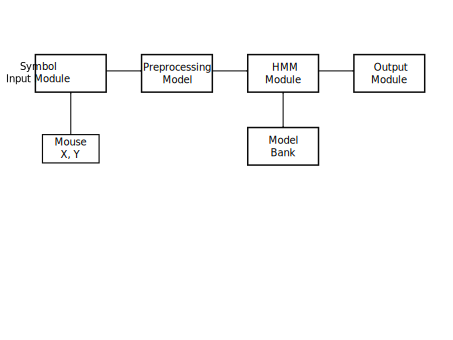
\includegraphics[width=0.80\textwidth]{graphics/demo-app/symbol-app-architecture-1.pdf}}%
	\only<2>{\centering \includegraphics[width=0.80\textwidth]{graphics/demo-app/symbol-app-architecture-2.pdf}}%
	\only<3>{\centering \includegraphics[width=0.80\textwidth]{graphics/demo-app/symbol-app-architecture-3.pdf}}%
	\only<4>{\centering \includegraphics[width=0.80\textwidth]{graphics/demo-app/symbol-app-architecture-4.pdf}}%
	
\end{frame}

\begin{frame}
	\frametitle{O aplicație simplă de recunoaștere a simbolurilor - Abordare (II)}
	Adaptare după \citep{yang1994hidden}.
	
	\begin{block}{Structura MMA}
		$N$(număr de stări) = 8\\
		2 variabile observabile de tip discrte per stare - $coef_{FFT}(x)$, $coef_{FFT}(y)$\\
		$M$(număr de valori pentru fiecare variabilă observabilă) = 256\\
		Modelul de tranziție:\\
		\begin{itemize}
			\item Bakis
			\item Ergodic
		\end{itemize}
	\end{block}
\end{frame}

\begin{frame}
	\frametitle{O aplicație simplă de recunoaștere a simbolurilor - Abordare (III)}
	
	Procedură de recunoaștere:
	\begin{enumerate}
		\item Construim și antrenăm câte un MMA pentru fiecare simbol în parte
		\vspace*{0.5em}
		\pause
		\item Folosim un set de date (simboluri) de validare pentru a stabili \emph{praguri} de recunoaștere, i.e. 
				dacă probabilitatea secvenței observate este prea mică pentru fiecare MMA, marcăm simbolul drept 
				\emph{necunoscut}
		\vspace*{0.5em}
		\pause
		\item Recunoaștere:
			\begin{itemize}
				\item Calculăm $P(O \vert \lambda_i)$ pentru fiecare MMA construit pentru simbolurile 
				$i=1,\cdots,nr\_simboluri$
				\item Alegem $\max(P(O \vert \lambda_i))$ ca și simbol candidat. 
				Daca $P(O \vert \lambda_i) > prag_i$, atunci am recunoscut \emph{simbolul i}, 
				altfel marcăm \emph{necunoscut}
			\end{itemize}
	\end{enumerate}
	
\end{frame}

\begin{frame}[t]
	\frametitle{O aplicație simplă de recunoaștere a simbolurilor - Rezultate}
	\scriptsize
	\begin{block}{Mărime set de date}
		\textbf{5} simboluri: \textbf{\emph{săgeată stânga, săgeată dreapta, cerc, pătrat, infinit}}\\
		\textbf{100} exemple per simbol: \textbf{50} antrenare, \textbf{10} validare, \textbf{40} testare
	\end{block}
	\normalsize
	
	\begin{columns}[T]
		\column{0.5\textwidth}
		\includegraphics[width=\textwidth]{graphics/demo-app/results-ergodic.png}
		\column{0.5\textwidth}
		\includegraphics[width=\textwidth]{graphics/demo-app/results-bakis.png}
	\end{columns}
\end{frame}